\chapter{Docker}
\section{安装docker和nvidia-docker}
安装docker:
\begin{lstlisting}[language = shell, numbers=left, 
		 numberstyle=\tiny,keywordstyle=\color{blue!70},
		 commentstyle=\color{red!50!green!50!blue!50},frame=shadowbox,
		 rulesepcolor=\color{red!20!green!20!blue!20},basicstyle=\ttfamily]
wget -O /etc/yum.repos.d/CentOS-Base.repo http://mirrors.aliyun.com/repo/Centos-7.repo  
yum install epel-release
yum install epel-release
yum install docker-ce
\end{lstlisting}

安装nvidia-docker
\begin{lstlisting}[language = shell, numbers=left, 
		 numberstyle=\tiny,keywordstyle=\color{blue!70},
		 commentstyle=\color{red!50!green!50!blue!50},frame=shadowbox,
		 rulesepcolor=\color{red!20!green!20!blue!20},basicstyle=\ttfamily]

distribution=$(. /etc/os-release;echo $ID$VERSION_ID)
curl -s -L https://nvidia.github.io/nvidia-docker/$distribution/nvidia-docker.repo | sudo tee /etc/yum.repos.d/nvidia-docker.repo

sudo yum install -y nvidia-container-toolkit
sudo systemctl restart docker
# Install nvidia-docker and nvidia-docker-plugin
wget -P /tmp https://github.com/NVIDIA/nvidia-docker/releases/download/v1.0.1/nvidia-docker-1.0.1-1.x86_64.rpm
sudo rpm -i /tmp/nvidia-docker*.rpm && rm /tmp/nvidia-docker*.rpm
sudo systemctl start nvidia-docker

# Test nvidia-smi
nvidia-docker run --rm nvidia/cuda nvidia-smi
\end{lstlisting}

\section{常用操作}
镜像(image)和容器(container)的关系,就像是面向对象程序设计中的类和实例一样,镜像是静态的定义,容器是镜像运行时的实体。容器可以被创建、启动、停止、删除和暂停等。

容器的实质是进程,但与直接在宿主机执行的进行不同,容器进程运行于属于自己的独立的命名空间。
\begin{lstlisting}[language = shell, numbers=left, 
		 numberstyle=\tiny,keywordstyle=\color{blue!70},
		 commentstyle=\color{red!50!green!50!blue!50},frame=shadowbox,
		 rulesepcolor=\color{red!20!green!20!blue!20},basicstyle=\ttfamily]
#开启镜像
sudo nvidia-docker run -it -v $(pwd)/DeepSpeech:/DeepSpeech -v /data1/asr_data:/mnt/data -v //data/kaldi/2019_0521_kaldi/kaldi-master:/mnt/kaldi paddlepaddle/deep_speech:latest-gpu /bin/bash
# 挂起镜像
Ctrl+P+Q
#运行已挂起的镜像
docker attach $CONTAINER_ID
\end{lstlisting}

\section{实践要求}
docker如果想要挂载上本地的IP地址,可以再运行docker的时候加上指令 --net=host。如果要挂载本地物理磁盘,加上指令 -v。如果要将宿主机的端口与容器的端口绑定,可以使用 -p <宿主机端口>:<容器端口>。
\begin{lstlisting}[language = shell, numbers=left, 
		 numberstyle=\tiny,keywordstyle=\color{blue!70},
		 commentstyle=\color{red!50!green!50!blue!50},frame=shadowbox,
		 rulesepcolor=\color{red!20!green!20!blue!20},basicstyle=\ttfamily]
nvidia-docker run -it --net=host  -p 50001:22 -v $(pwd)/DeepSpeech:/DeepSpeech  -v /data1/asr_data:/mnt/data -v /data/kaldi/2019_0521_kaldi/kaldi-master:/mnt/kaldi duhu/ds-server /bin/bash
docker commit <image-id> <new-image-name> \\保存修改后的镜像
-a :提交的镜像作者;
-c :使用Dockerfile指令来创建镜像;
-m :提交时的说明文字;
-p :在commit时,将容器暂停。
将容器a404c6c174a2 保存为新的镜像,并添加提交人信息和说明信息。
docker commit -a "runoob.com" -m "my apache" a404c6c174a2 mymysql:v1
#保存镜像到本地,存下来的文件可以用于在不同的主机之间转移镜像
docker save ubuntu | gzip > ubuntu-latest.tar.gz \\保存镜像
zcat ubuntu-latest.gz | docker import - ubuntu:latest \\导入镜像
docker run -i -t ubuntu /bin/bash \\运行镜像

\end{lstlisting}

\href{https://juejin.im/post/5badee89e51d450e6160312a}{解决docker容器存放目录磁盘空间满了问题
}

\begin{enumerate}
  \item 容器不应该向其存储层内写入任何数据,容器存储层要保持无状态化。所有的文件写入操作,都应该使用数据卷(Volume)、或者绑定宿主目录,在这些位置的读写会跳过容器存储层,直接对宿主(或网络存储)发生读写,其性能和稳定性更高。
  \item 数据卷的生存周期独立于容器,容器消亡,数据卷不会消亡。因此,使用数据卷后,容器删除或者重新运行之后,数据却不会丢失。
\end{enumerate}

\section{docker安装TensorFlow}
为了避免影响到主机上诸多配置,因此选用docker安装TensorFlow,想怎么造就怎么造。安装TensorFlow时,使用以下指令就会启动该镜像安装。
\begin{lstlisting}[language = shell, numbers=left, 
		 numberstyle=\tiny,keywordstyle=\color{blue!70},
		 commentstyle=\color{red!50!green!50!blue!50},frame=shadowbox,
		 rulesepcolor=\color{red!20!green!20!blue!20},basicstyle=\ttfamily]
docker pull  tensorflow/tensorflow
\end{lstlisting}


\section{docker乱七八糟的错误}
在使用\textcolor{magenta}{docker build - < Dockerfile}指令进行镜像安装的时候,如果多次执行这个指令,由于这个镜像有一个默认的tag,所以第二次及后续多次安装都无法使用这个tag,这个tag在第一次安装的时候已经被使用了,这就一会导致出现一堆的\textcolor{magenta}{<none> <none>}的镜像,如图\ref{fig:docker-tag-none}。
\begin{figure}[htbp]
  \centering
  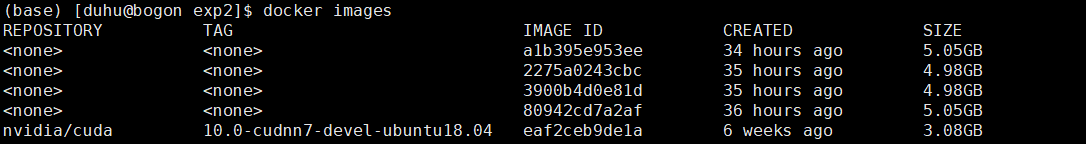
\includegraphics[width=0.9\textwidth]{docker-tag-none}
  \caption{Docker重复安装出现<none>:<none> \label{fig:docker-tag-none}}
\end{figure}

参考\href{https://stackoverflow.com/questions/30179716/what-are-none-repository-and-tags-why-do-they-appear-when-i-use-docker-build}{这里},那在这种情况下,首先我们可以使用指令\textcolor{magenta}{docker rmi \$(docker images -f "dangling=true" -q)}去除掉所有的无效镜像。
然后使用指令\textcolor{magenta}{docker rmi <REPOSITORY>:<TAG>}来删掉所有的镜像,然后重新安装,重新安装的时候,使用指令\textcolor{magenta}{docker build -t <REPOSITORY>:<TAG> -< Dockerfile}。